O objetivo deste primeiro capítulo é mostrar-lhe os fundamentos essenciais sobre o mundo da programação. Começaremos por utilizar pseudocódigo (conceito explicado à frente), avançando gradualmente até chegar à linguagem pretendida: a Linguagem C.

\section{Linguagens de programação}

À semelhança de uma linguagem humana, uma linguagem de programação permite-nos comunicar, não com Humanos, mas com computadores ou qualquer outro sistema computorizado. Linguagens de programação são constituídas por uma \quotes{gramática} que contém todas as regras sintáticas utilizadas. Através da utilização dessas regras, podemos comunicar instruções a um computador, ou seja, instruir-lhe a fazer algo. É assim que os programas são criados.

\begin{defi}
\textbf{Regras sintáticas} consistem num conjunto de normas a seguir que indicam como se deve estruturar o código, ou seja, como se deve construir o código.
\end{defi}

Existem inúmeras linguagens de programação: algumas de propósito geral, ou seja, sem ter uma finalidade específica. Por outro lado, existem outras criadas para um domínio específico. A linguagem de programação C é um exemplo de uma linguagem de programação de propósito geral. Por outro lado a \textit{Wolfram Language}\footnote{Consultar \color{links}\href{http://www.wolfram.com/language/}{wolfram.com/language}}, é uma linguagem de domínio específico, multi-paradigma (abordado mais à frente) e dedicada à Matemática. 

\section{Algoritmos}

É importante compreender alguns conceitos básicos que serão fundamentais na sua jornada no mundo da programação. Assim, vai começar por entender o que são \textbf{algoritmos} visto que vai estar sempre em contacto com eles.

\begin{defi}
\textbf{Algoritmos} são quaisquer sequências de instruções finitas e bem definidas que podem ser executadas por computadores, autómatos ou até mesmo humanos.
\end{defi}

Na Figura 1.1 pode visualizar todo o processo da confeção de um bolo onde o algoritmo é a receita – uma sequência de instruções bem definida e finita – que é executada pelo(a) \quotes{cozinheiro(a)}.

\begin{figure}[!htbp]
\center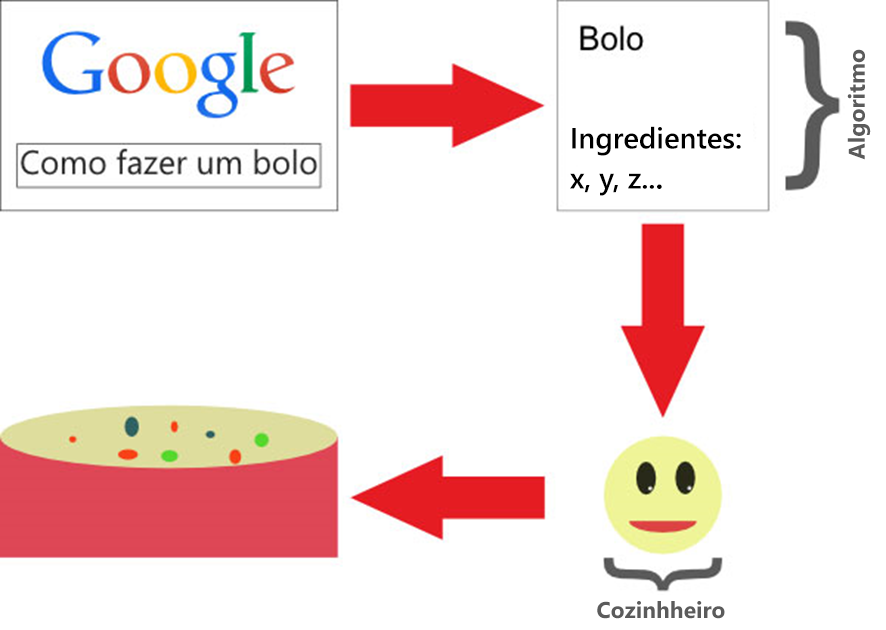
\includegraphics[scale=0.5]{images/confecao_bolo.png}
\caption{Confeção de um bolo}
\end{figure}

Os algoritmos podem ser representados de diversas formas. Aqui são abordadas duas delas: os fluxogramas e o pseudocódigo. Estas representações dos algoritmos são essenciais antes destes serem escritos em código; ir-se-à poupar tempo visto que são reduzidos os possíveis erros durante o desenvolvimento.

Nem sempre são precisos os dois tipos de representação de algoritmos. Por vezes basta um. Isso é algo que depende do fluxo e métodos de trabalho de cada pessoa. Os fluxogramas e pseudocódigo são algo universal, que não se compromete com uma determinada linguagem de programação.

\subsection{Fluxogramas}

Vejamos então a primeira forma de representar algoritmos, os fluxogramas.

\begin{defi}
Um \textbf{fluxograma} é uma representação gráfica de um algoritmo que utiliza símbolos de forma a demonstrar os processos neste realizado.
\end{defi}

Existem várias vantagens na criação de fluxogramas como, por exemplo, a sua facilidade de criar, a facilidade na partilha e ajuda a criar modelos mentais.

Um fluxograma pode fazer uso de muitos símbolos. No entanto, apenas iremos necessitar dos básicos para ter uma boa compreensão de como funcionam os fluxogramas. Pode visualizar estes símbolos na Figura 1.2.

\begin{figure}[!htbp]
\center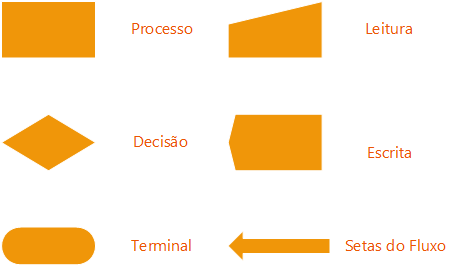
\includegraphics[scale=0.65]{images/simbolos.png}
\caption{Símbolos primários dos fluxogramas}
\end{figure}

Na Figura 1.3 pode visualizar um fluxograma, baseado no processo de confeção de um bolo.

\subsection{Pseudocódigo}

Uma forma mais aproximada do código final é a utilização de pseudocódigo. Sendo assim, sucede a criação dos fluxogramas.

\begin{defi}
\textbf{Pseudocódigo} é uma forma de representação de algoritmos que se assemelha a linguagens de programação mas que utiliza a língua nativa do utilizador de forma a ser facilmente entendida por quem não tem quaisquer conhecimentos da sintaxe de uma linguagem de programação.
\end{defi}

Os programadores cuja língua nativa é português, costumam referir-se ao pseudocódigo como \textit{Portugol}, também conhecido por \quotes{Português Estruturado}. O seguinte trecho de Portugol representa o algoritmo anteriormente representado com um fluxograma, a confeção de uma receita: 

\begin{lstlisting}
inicio      
   variavel caracter receita <- "A minha receita"      
 
  se tenhoIngredientes(receita) == verdadeiro entao      
      fazerBolo()      
  senao      
      comprarIngredientes()      
      fazerBolo()      
 fimse      
fim
\end{lstlisting}
   
Como pode verificar, o algoritmo acima, em Portugol, é extremamente simples de compreender. De momento, peço-lhe que entenda as expressões que terminam com \texttt{()} como se fossem comandos.

\begin{defi}
Um \textbf{comando} é uma ordem ou instrução dada a um computador ou qualquer outra máquina automatizada.
\end{defi}

\begin{figure}[!htbp]
\center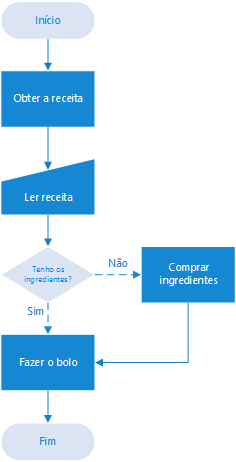
\includegraphics[scale=0.75]{images/confecao_bolo_al.png}
\caption{Fluxograma \quotes{Confeção de um bolo}}
\end{figure}

\section{Constantes e variáveis}

Na quarta linha do trecho de código que visualizou em \textbf{1.2.2}, pôde encontrar o seguinte código:

\begin{lstlisting}
variavel caracter receita <- "A minha receita"    
\end{lstlisting}

Esse trecho de código declara uma variável do tipo \textbf{caracter}, que se chama \texttt{receita}, com o valor \quotes{A minha receita}.

\begin{defi}
A \textbf{declaração de variáveis}, ou constantes, consiste no processo em que o compilador é "avisado" da sua existência para que, de cada vez se menciona o nome da variável/constante, esta seja utilizada.
\end{defi}

Por exemplo, quando declaramos a variável \texttt{receita}, estamos a reservar um endereço da memória RAM para alocar um valor. Neste caso, o valor foi atribuído no momento da sua declaração utilizando o operador \quotes{$\leftarrow$} (sem aspas).

A partir do momento declaramos uma variável ou constante, o endereço da memória RAM que foi reservado estará disponível através do seu nome. Sempre que for referenciado \texttt{receita} no código, o valor da variável será retornado.

\subsection{Constantes}

Comecemos por abordar as constantes.

\begin{defi}
\textbf{Constantes} permitem armazenar valores imutáveis, ou seja, que não podem ser alterados ao longo da execução de um programa.
\end{defi}

Ora veja o seguinte exemplo:

\begin{lstlisting}
constante caracter EMPRESA <- "Pplware"    
EMPRESA <- "A Minha Empresa"   
\end{lstlisting}

Na primeira linha, a constante \texttt{EMPRESA}, do tipo carácter, é declarada e é-lhe atribuído o valor \texttt{Pplware}. De seguida, na segunda linha, existe uma tentativa de alterar o seu valor da constante. Esta tentativa irá falhar, causando um erro visto que o valor de uma constante não pode ser alterado após a sua atribuição.

\begin{mdframed}[backgroundcolor=cinzaclaro, linewidth=0pt]
\textbf{Nomenclatura} 

Convencionalmente, o nome das constantes é escrito com letras maiúsculas para haver uma melhor distinção no código-fonte. Esta convenção não é obrigatória e não irá causar quaisquer erros durante a execução de um programa. Seguir esta convenção apenas torna mais clara a distinção entre variáveis e constantes dentro do código-fonte facilitando tanto a si, como programador, como a outros programadores que vejam o código do seu programa.
\end{mdframed}

\subsection{Variáveis}

Por outro lado, existem as variáveis.

\begin{defi}
\textbf{Variáveis}, ao contrário das constantes, permitem o armazenamento de valores que podem ser alterados durante a execução de um programa. Geralmente são utilizadas para manter estados de algo e são fundamentais na programação.
\end{defi}

Abaixo encontra um exemplo:

\begin{lstlisting}
variavel caracter temaDaSecao <- "Constantes"      
temaDaSecao <- "Variáveis"  
\end{lstlisting}

Na primeira linha é declarada uma variável do tipo carácter, com nome \texttt{temaDaSecao} e valor \texttt{Constantes}. Seguidamente, o seu valor é alterado para \texttt{Variáveis} não causando nenhum erro, pois o valor das variáveis pode ser alterado ao longo da execução de um programa.

\paragraph{Regras de nomeação}

Existem diversas regras que têm de ser seguidas no momento da declaração de uma variável para que não seja causado nenhum erro.

O nome das variáveis e constantes:

\begin{itemize}
  \item Não pode começar com números (ex.: \texttt{9comida} não é permitido, \texttt{comida9} é válido);
  \item Não pode ser igual a uma palavra reservada (ex.: \texttt{if} não é permitido, mas \texttt{maria} é permitido);
  \item Não pode conter espaços (ex.: \texttt{a minha var} não é permitido, porém \texttt{aMinhaVar} é válido);
  \item Não pode conter caracteres especiais (existem exceções em diversas linguagens).
\end{itemize}

\begin{defi}
\textbf{Palavras reservadas} são aquelas que constam na gramática da linguagem de programação. Tendo em conta que a palavra \quotes{se} é um comando do Portugol, não podemos declarar nenhuma variável ou constante com esse nome. Se isso for feito, será gerado um erro.
\end{defi}

As variáveis e constantes podem ser de diversos tipos. Os tipos de dados existentes variam de linguagem para linguagem. Mais à frente irão ser abordados os tipos de dados na linguagem C.

\begin{mdframed}[backgroundcolor=cinzaclaro, linewidth=0pt]
\textbf{Nomenclatura} 

As variáveis, ao contrário das constantes, não são totalmente escritas em letras maiúsculas. Convencionalmente, a variação \textit{lowerCamelCase} (pertencente ao padrão \textit{CamelCase}) é seguida na maioria das linguagens de programação. Este padrão será utilizado visto que a maioria das linguagens de programação adotam-no, tal como a linguagem C.
\end{mdframed}

\section{Paradigmas de programação}

Todas as linguagens de programação têm características que as distinguem de outras. O(s) paradigma(s) de programação que ela segue são fundamentais.

\begin{defi}
\textbf{Paradigmas de programação} são modelos ou padrões da forma de estruturar o nosso código. Existem muitos. 
\end{defi}

Nesta secção apenas são abordados 6 paradigmas de programação, os mais conhecidos e utilizados. As que adotam mais do que um paradigma chamam-se \textbf{multi-paradigma}.

\subsection{Paradigma imperativo}

O primeiro paradigma abordado é o paradigma imperativo. Este concentra-se num \textbf{estado} (que são as variáveis) e em \textbf{ações} (comandos) que \textbf{modelam} (alteram) esse estado.

Este paradigma pode ser comparado ao modo imperativo da linguagem humana visto que é criado para ordenar a realização de ações (como por exemplo, fazer algo, recortar, analisar, apagar...).

Alguns \textbf{exemplos} de linguagens de programação imperativas são, por exemplo: C, Java, C\#, Pascal.

\subsection{Paradigma procedimental}

Com o paradigma procedimental, trechos de código podem ser reutilizados sem a necessidade de o copiar para diversos locais através da utilização de funções e procedimentos (que serão abordados mais a frente). 

A maioria das linguagens de programação adotam este paradigma. 

\subsection{Paradigma estruturado}

Nas linguagens de programação em que o paradigma estruturado é seguido, o código-fonte de uma aplicação pode ser reduzido em apenas três estruturas: sequência, decisão e iteração (repetição).

\paragraph{Sequência}

Nesta primeira estrutura, as tarefas são executadas de forma linear, ou seja, uma após a outra. Abaixo encontra um pequeno exemplo.

\begin{lstlisting}
Acordar;        
Vestir;        
Tomar o pequeno-almoco;        
Ir trabalhar;  
\end{lstlisting}

Este é um exemplo de uma sequência onde são realizadas as ações normais do dia-a-dia de um indivíduo que está empregado.

\begin{figure}[!h]
\center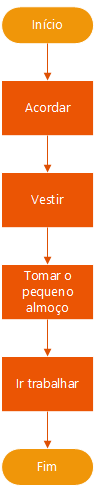
\includegraphics[scale=0.75]{images/sequencia.png}
\caption{Fluxograma de uma sequência}
\end{figure}

Na maioria das linguagens de programação, os comandos/ações terminam com ponto e vírgula pois estas permitem que os comandos sejam colocados em linha da seguinte forma:

\begin{lstlisting}
Acordar; Vestir; Tomar o pequeno-almoco; Ir trabalhar; 
\end{lstlisting}

A utilização do ponto e vírgula é normalmente obrigatória quando existe mais do que uma instrução numa só linha. Existem linguagens de programação que só obrigam a utilização de ponto e vírgula nestes casos (JavaScript, por exemplo). Porém, existem outras, como C, Java e C\# que obrigam a utilização de ponto e vírgula no final de \textbf{todas} as instruções.

\paragraph{Decisão}

Neste tipo de estrutura, existe um trecho de código que é executado ou não dependendo do resultado de um teste lógico, também conhecido por predicado. Abaixo encontra diversos exemplos para esta estrutura.

O exemplo abaixo descreve a condição/decisão \quotes{Se acordar, vou trabalhar. Caso contrário, não vou trabalhar} (em pseudocódigo).

\begin{lstlisting}
if "Acordar" then        
  "Trabalhar"        
else      
  "Não trabalhar"        
endif   
\end{lstlisting}

\textit{\textbf{Novos Termos:}}

\begin{itemize}
	\item \textbf{if} \(\rightarrow\) se
	\item \textbf{then} \(\rightarrow\) então
	\item \textbf{else} \(\rightarrow\) caso contrário
	\item \textbf{endif} \(\rightarrow\) fim do se
\end{itemize}

O pseudocódigo acima já não está em português; já não é Portugol. O que encontra acima já se assemelha ao que irá visualizar nas linguagens de programação.

Retornando novamente ao trecho de código escrito acima, repare que \texttt{Trabalhar} só será executado se e apenas se o indivíduo \texttt{Acordar}. Caso contrário, o trecho \texttt{Não trabalhar} será executado.

\begin{figure}[!h]
\center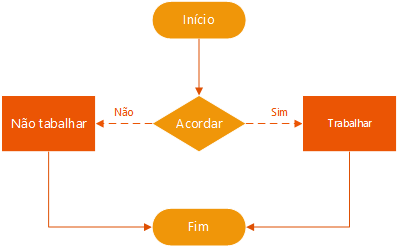
\includegraphics[scale=0.75]{images/decisao01.png}
\caption{Exemplo de uma decisão em fluxograma}
\end{figure}
 
Agora veja o seguinte exemplo em que a condição \quotes{Dói-me a cabeça. Se doer muito pouco, vou trabalhar. Se doer pouco, tomo um comprimido e vou trabalhar. Se doer muito, vou ao médico e falto ao trabalho} é executada.

\begin{lstlisting}
case "Dor de cabeca"        
  when "muito pouco" then "trabalhar"        
  when "pouco" then "tomar comprimido"; "trabalhar"        
  when "muito" then "ir ao médico"; "não trabalhar"    
\end{lstlisting}

\textit{\textbf{Novos Termos:}}

\begin{itemize}
\item \textbf{case} \(\rightarrow\) caso
\item \textbf{when} \(\rightarrow\) quando
\item \textbf{else if} \(\rightarrow\) caso contrário se
\end{itemize}

\begin{figure}[!h]
\center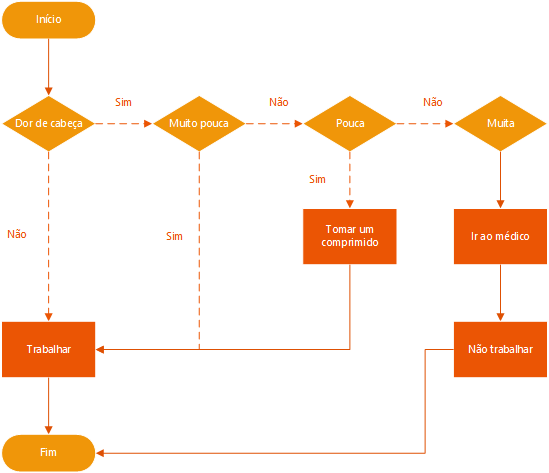
\includegraphics[scale=0.75]{images/decisao02.png}
\caption{O que farei se me doer a cabeça}
\end{figure}

Este é mais um exemplo mas utilizando diferentes comandos. Este trecho poderia ser também escrito através de \textit{primitivas if/else} da seguinte forma (ver Figura 1.6):

\begin{lstlisting}
if "Dor de cabeca"          
  if "muito pouco" then          
    "trabalhar";          
  else if "pouco" then          
    "tomar comprimido";          
    "trabalhar";          
   else if "muito" then          
    "ir ao médico";          
    "não trabalhar";          
   endif          
endif      
\end{lstlisting}
 
\paragraph{Iteração}

Neste tipo de estrutura, também conhecido como repetição, um trecho de código é repetido um número finito de vezes dependendo do resultado de um teste lógico. 

Abaixo encontra a repetição \quotes{não saio de casa enquanto não estiver vestido} em pseudocódigo:

\begin{lstlisting}
do {        
  "não sair de casa";        
} while ( "não estou vestido" )     
\end{lstlisting}

\textit{\textbf{Novo termo:}}
\begin{itemize}
\item \textbf{do} \(\rightarrow\) fazer
\end{itemize}

Ou seja, o código acima pode ser lido da seguinte forma: \textbf{fazer} \quotes{não sair de casa} \textbf{enquanto} \quotes{não estou vestido}. De forma generalizada, fazer x enquanto y.

Agora veja o retrato da repetição \quotes{enquanto durmo, não me visto} em pseudocódigo:

\begin{lstlisting}
while ( durmo )        
 naoMeVisto();       
\end{lstlisting}

Ou seja, \textbf{enquanto} acontece algo, faço outra coisa. 

Visualize agora o código correspondente à ação \quotes{lavar os dentes 20 vezes}.

\begin{lstlisting}
for ( i = 0; i++; i < 20 )        
  lavarOsDentes();      
\end{lstlisting}

Ou seja, enquanto não acontece qualquer coisa, faço qualquer coisa.

Mais um exemplo, mas referente à expressão \quotes{Para cada dente, lavo-o muito bem}.

\begin{lstlisting}
for each dente in boca        
 lavarMuitoBem();    
\end{lstlisting}

\textit{\textbf{Novos Termos:}}

\begin{itemize}
\item \textbf{each} \(\rightarrow\) cada
\item \textbf{in} \(\rightarrow\) em
\end{itemize}

Ou seja, para cada item do conjunto, fazer qualquer coisa.

\subsection{Paradigma declarativo}

O Paradigma Declarativo contrasta com o Imperativo pois é capaz de expressar a lógica sem descrever como o fluxo de comandos funciona, ou seja, apenas diz ao computador \textbf{o que} fazer e não \textbf{como} fazer. 

Um excelente \textbf{exemplo} de uma linguagem que utiliza este paradigma é Prolog, muito utilizado na área de inteligência artificial.

\subsection{Paradigma funcional}

O Paradigma Funcional engloba todas as linguagens de programação que utilizam funções matemáticas e evita estados. Estas linguagens de programação são muito utilizadas no campo da matemática. 

Algumas linguagens que seguem o paradigma funcional são, por \textbf{exemplo}, Matlab, Wolfram Language, B.

\subsection{Paradigma orientado a objetos}

A Programação Orientada a Objetos permite a criação de \textbf{objetos} com base em \textbf{classes}. Estes objetos são instâncias dessas classes e possuem todos os atributos e funções presentes nas classes em questão. 

Este paradigma é muito extenso e tem muita informação que mais à frente irá ser abordada. Atualmente existem muitas linguagens que utilizam este paradigma (Java, C++, C\#, PHP, por exemplo). 

\vspace{1em}

Os paradigmas de programação não se limitam aos 6 (seis) apresentados pois existem inúmeros outros. Estes são apenas os paradigmas de programação mais abrangentes. Existem paradigmas baseados noutros paradigmas, outros que contrastam com outros, etc.

\section{A linguagem C}

Os anos de 1969 a 1973 foram de extremo entusiasmo dentro da AT\&T Bell Labs porque foi quando a linguagem de programação C \textbf{foi maioritariamente desenvolvida}.

O principal desenvolvedor desta linguagem foi \textbf{Dennis Ritchie} que descreveu o ano de 1972 como o mais produtivo e criativo.

\begin{figure}[!h]
\center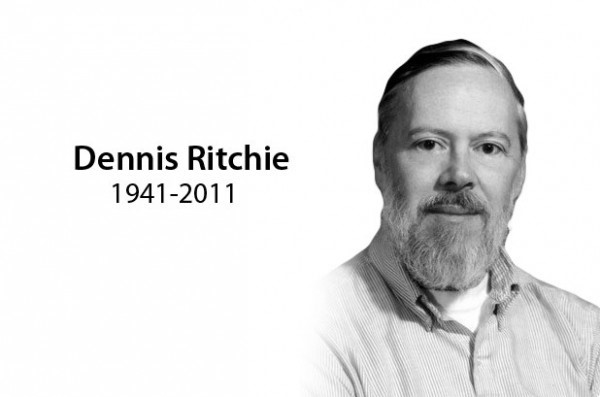
\includegraphics[scale=0.75]{images/dennisritchie.jpg}
\caption{Dennis Ritchie}
\end{figure}

A linguagem desenvolvida por Ritchie chama-se \textbf{C} porque esta linguagem baseou-se imenso numa outra linguagem de programação chamada \textbf{B}, tendo C diversas características em comum com B.

Inicialmente, esta linguagem de programação, C, tinha como principal finalidade o desenvolvimento do Unix, que já havia sido escrito em \textbf{Assembly} - uma outra linguagem de programação.

A versão mais recente de C é C11 e foi lançada a dezembro de 2011. Esta linguagem foi uma das influências de muitas das linguagens de programação que atualmente são muito utilizadas. Entre muitas outras, C influenciou AWK, BitC, C++, C\#, C Shell, D, Euphoria, Go, Java, JavaScript, Limbo, Logic Basic, Objective-C, Perl e PHP. \textbf{Isto não significa que estas linguagens não tenham sido influenciadas por outras.}

Nós iremos começar por abordar C porque é uma linguagem \quotes{mãe}, que influenciou muitas outras. Por ser uma linguagem de baixo nível, pode ter um contacto mais próximo com o \textit{hardware}.

\subsection{Características da linguagem C}

Como abordámos anteriormente, os paradigmas de programação são muito importantes e influenciam a forma como devemos escrever.

C é uma linguagem de programação, em relação aos paradigmas, \textbf{estruturada}, \textbf{imperativa} e \textbf{procedimental}. Outras características desta linguagem são o facto de ser padronizada pela ISO e de propósito geral.

\paragraph{Linguagem de programação compilada}

Linguagens de Programação Compiladas são aquelas que passam pelo processo de compilação, ou seja, onde o seu código fonte é diretamente transformado na linguagem da máquina por via de um compilador.

\begin{defi}
\textbf{Código fonte} é um conjunto de instruções lógicas, escritas de acordo com uma linguagem de programação existente.
\end{defi}

\begin{figure}[!h]
\center
\includegraphics[scale=4]{images/lang.jpg}
\caption{Linguagem C}
\end{figure}

Aprendendo a linguagem C, fica preparado para se iniciar com muitas outras linguagens de programação pois tem uma sintaxe muito utilizada e, além disso, sabe a lógica.

\subsection{Ambiente de desenvolvimento}

Para começar a desenvolver programas, necessita ter um ambiente de desenvolvimento, preparado com as diversas ferramentas necessárias.

\subsubsection{Instalação de um compilador}

\begin{defi}
Um \textbf{compilador} é a ferramenta que transforma o código-fonte na linguagem da máquina através do processo de compilação.
\end{defi}

O compilador que iremos utilizar denomina-se GCC (\textit{GNU Compiler Collection}). Este compilador é de fácil instalação e utilização.

\paragraph{Debian e derivadas} 

A instalação deste compilador na distribuição Linux Debian ou derivadas, como por exemplo, Ubuntu, é bastante simples. No terminal, execute os seguintes comandos:

\begin{lstlisting}[language=bash,numbers=none]
> sudo apt-get update && apt-get upgrade
> sudo apt-get install build-essential
\end{lstlisting}

Depois desses dois comandos deverá ter instalado o compilador GCC, entre outras ferramentas. Para verificar se o GCC ficou instalado corretamente execute, o seguinte comando:

\begin{lstlisting}[language=bash,numbers=none]
> gcc -v
\end{lstlisting}

Este comando deverá retornar a versão atualmente instalada do GCC.

\paragraph{Outras distribuições Linux}

Para outras distribuições Linux é recomendável seguir as instruções encontradas na página oficial do projeto GCC\footnote{Ver \color{links}\href{https://gcc.gnu.org/}{gcc.gnu.org}}.

\paragraph{Windows}

No sistema operativo da Microsoft, o GCC pode ser instalado recorrendo a projetos como o MinGW ou o Cygwin. Recomendo o primeiro\footnote{\textit{Download} em \color{links}\href{http://www.mingw.org/download/installer?}{mingw.org/download}}.

\paragraph{OS X}

No sistema operativo da Apple, o GCC costuma vir com o Xcode, um IDE multi-linguagem criado pela Apple, podendo tudo isto ser instalado através do terminal com o seguinte comando:

\begin{lstlisting}[language=bash,numbers=none]
> xcode-select --install
\end{lstlisting}

Pode verificar a versão instalada do GCC nos dois últimos sistemas operativos recorrendo ao comando anteriormente mencionado.

\begin{mdframed}[backgroundcolor=cinzaclaro, linewidth=0pt]
Um \textbf{IDE} é um Ambiente de Desenvolvimento Integrado, do inglês \textit{Integrated
Development Environment}. É um programa de computador que reúne diversas ferramentas
para apoiar no desenvolvimento de software.
\end{mdframed}

\subsubsection{Editor de texto}

Além do compilador, irá também precisar de um editor de texto. Qualquer editor de texto funciona, mas recomendo um que suporte a sintaxe da linguagem C.

Existem vários editores de texto que pode utilizar. Aqui deixamos algumas recomendações:

\begin{itemize}
\item \textbf{Windows} \(\rightarrow\) Notepad++, Atom, Sublime Text;
\item \textbf{Linux} \(\rightarrow\) Gedit, Atom, Sublime Text (algumas distribuições), Vim;
\item \textbf{OS X} \(\rightarrow\) TextWrangler, Sublime Text, Atom.
\end{itemize}

\subsection{\quotes{Hello World!}}

Como seria o mundo da programação sem o famoso \quotes{Hello World}? É uma tradição o primeiro programa criado por alguém imprimir a mensagem \quotes{Hello World} no ecrã.

Crie um ficheiro, onde queira, com o nome HelloWorld.c. Tenha em atenção à extensão do ficheiro que tem que ser .c, ou seja, da linguagem C.

Abra esse mesmo ficheiro com um editor de texto, copie e cole o seguinte texto e então guarde as alterações.

\begin{lstlisting}
#include <stdio.h>      
#include <stdlib.h>
       
int main() {
  printf("Hello World!\n");      
  return 0;
}
\end{lstlisting}

Este trecho de código irá imprimir no ecrã a mensagem \quotes{Hello World!}. Para executarmos este comando, deverá abrir a Linha de Comandos/Terminal e navegar até ao local onde guardou o ficheiro. Depois, execute o seguinte comando:

\begin{lstlisting}[language=bash,numbers=none]
> gcc HelloWorld.c -o HelloWorld
\end{lstlisting}

Onde HelloWorld.c é o ficheiro de entrada e HelloWorld o ficheiro de saída. A extensão do ficheiro produzido deverá ser diferente consoante o sistema operativo.

No meu caso, como estou a utilizar o Windows, foi criado um ficheiro \textbf{.exe}. Agora, para executar o seu ficheiro, basta o executar através da linha de comandos:

\begin{lstlisting}[language=bash,numbers=none]
> HelloWorld
\end{lstlisting}

Deverá receber uma mensagem na Linha de Comandos a dizer \quotes{Hello World}.

\subsection{\texttt{\#include}}

A primeira linha do trecho acima \textbf{não} é C mas sim uma indicação para o \textbf{compilador}. 

\begin{mdframed}[backgroundcolor=cinzaclaro, linewidth=0pt]
C é uma linguagem utilizada em locais que necessitam de alta velocidade, como o \textit{kernel} - núcleo - do Linux, pois esta tem essa capacidade.

Devido à alta velocidade que pode ser proporcionada por esta linguagem, C não está preparado, por omissão, para todos os tipos de tarefas. Assim, precisamos de incluí-las para ter disponíveis mais funções.
\end{mdframed}

A linguagem C não vem \quotes{empacotada} de funções por padrão e é necessário incluí-las. Para as incluir, utilizamos a diretiva \texttt{\#include} que diz ao compilador que precisa de incluir ficheiros ponto H (.h) que são ficheiros do tipo \textit{header}.
Nesta caso adicionámos o ficheiro \texttt{stdio.h} que quer dizer \textit{standard input/output}, ou seja, sistema padrão de entrada e saída.

\subsection{Função \texttt{main}}

Todos os programas C têm que ter, obrigatoriamente, uma função \texttt{main} que será automaticamente executada. Esta função é o ponto de partida para criar um programa. É o seu cerne.

Voltaremos a falar sobre este tema e da sua importância.

\subsection{Função \texttt{printf}}

Este é um comando/função que está contido no ficheiro stdio.h. Caso não incluamos o ficheiro, será gerado erro. Esta função significa \textit{print formatted}, ou seja, \quotes{escrita de dados formatados}.

Esta função aceita vários parâmetros; permite-nos enviar várias coisas que irão ser processadas por ela. De momento, apenas iremos falar do primeiro argumento.

O primeiro argumento é uma \textit{string}, ou seja, um conjunto de caracteres. Este conjunto de caracteres deve ser colocado dentro de aspas.

Neste caso escrevemos \texttt{Hello World!\textbackslash n!} o que quer dizer que será imprimido \quotes{Hello World!} na janela. E o que faz \texttt{\textbackslash n}? Simples, é um carácter especial que imprime uma nova linha. Chama-se \textit{new line}.

A \texttt{\textbackslash} serve para inserir caracteres especiais.

\begin{table}[h]
\center\begin{tabular}{|l|l|}
\hline
\texttt{\%\%}     & Por cento                                            \\ \hline
\texttt{\textbackslash t}      & Tab                                                  \\ \hline
\texttt{\textbackslash r}      & Carriage Return (coloca o cursor no início da linha) \\ \hline
\texttt{\textbackslash a} e \textbackslash 7 & Alguns sons                                          \\ \hline
\end{tabular}
\caption{Alguns caracteres especiais em C}
\end{table}

\subsection{\texttt{return}}

Como referi acima, a função \texttt{main} irá, neste caso, retornar um número inteiro. É aqui que o comando \textit{return}, que quer dizer retorno, entra. Este retorna o número 0 que é o \textbf{binário para falso}.

De momento, ainda não temos muito a acrescentar sobre esta diretiva mas mais à frente iremos falar de novo sobre ele quando abordarmos funções e procedimentos.

\subsection{Comentários}

Os comentários, em programação, são colocados para auxiliar ou dar mais informações sobre alguma parte ou trecho do código. Os comentários são completamente ignorados pelo compilador.

Os comentários que iniciam por \quotes{//} começam nesse local e prolongam-se até ao final da linha em questão. Os blocos de comentários maiores começam por \quotes{/*} e terminam com \quotes{*/} e tudo o que está contido entre eles é um comentário.

Estes não devem ser utilizados para coisas óbvias como, por exemplo, \quotes{aqui somam-se as variáveis a e b}. Devem-se utilizar os comentários de dupla barra em variáveis e constantes (ou para comentários curtos). Para comentar algo mais longo como funções ou classes, deverá ser utilizada a estrutura \quotes{*/}.

\begin{lstlisting}
#include <stdio.h>    
     
int main() {        
    int n = 1; //Até ao final da linha é um comentário.    
     
    /*  
     TUDO ISTO é um comentário            
     */   
}    
\end{lstlisting}

Em C, o tipo de comentários mais utilizado é aquele que começa por \quotes{/*}, independentemente do tamanho do comentário.